\chapter{Database and Data Modeling}

	The database model is described, in this chapter. It's a fairly simple model although additions can be made to augment and improve the application's features.

	\begin{figure}[h!]
		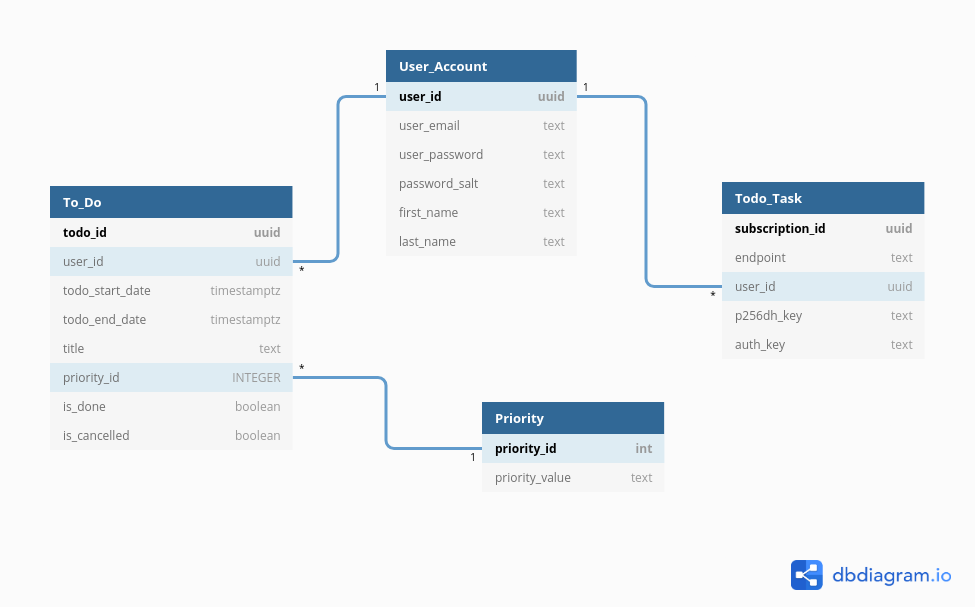
\includegraphics[width=17cm,scale=0.6]{./images/data_model_2do}
		\caption{Data Model}
	\end{figure}

	A user can have multiple to-do's and subscriptions (tasks). The need for multiple subscriptions stems from the fact that the user can have multiple instances of the application running in different desktops.\\
	There also is a priority system which hasn't yet been implemented. In the future each to-do will have a priority with a specific value and this value will be used to calculate how many times the user will be notified.
	